\input{../../../common/preamble.tex}
\input{../../../common/preamble-addon-envs.tex}
\input{../../../common/preamble-addon-listings.tex}
\usepackage{url}
\usepackage{etex}
\usepackage{tikz,pgfplots}
\pgfplotsset{compat=1.9}

% For importing mixed pdf-tex files
\usepackage{import}


\author{Einar Baumann}
\title{
    \vspace{-1in}
    \usefont{OT1}{bch}{b}{n}
    \normalfont \normalsize \textsc{TKT4140 Numeriske beregninger med datalab} \\ [20pt]
    \vspace{0.1in}
    \rule{\textwidth}{0.5pt} \\[1cm]
    {\sffamily \huge Numerisk løsing av randverdiproblemer med skyteteknikk} \\
    \vspace{0.1in}
    \rule{\textwidth}{2pt} \\[0.7cm]
}

\begin{document}
\maketitle
\thispagestyle{empty}
\clearpage

\section{Lineære ligninger} % (fold)
\label{sec:line_re_ligninger}
Skyteteknikk er en metode til å transformere et randverdiproblem for en ODL til et ekvivalent initialverdiproblem.\cite{komp}. Metodens navn stammer fra problemstillingen skissert i Figur~\ref{fig:skyting}.

Mer spesifikt så fungerer metoden ved at man ser på rabndbetingelsene som en funksjon av initialbetingelser i et punkt -- dette reduserer randverdiproblemet til å finne initialbetingelsene som gir en rot.

I Figur~\ref{fig:skyting} vil vi finne vinkelen $\alpha$ som gir skytelengden $x=L$. Vi kjenner her betingelsene for $x=0$ og $x=L$, og det er innlysende at problemet kan løses ved å variere $\alpha$.

\begin{figure}[htbp]
  \centering
  \import{graphics/}{shooting.pdf_tex}
  \caption{Illustrasjon av skyting.}
  \label{fig:skyting}
\end{figure}

\subsection{Bestemmelse av randverdi vha. interpolasjon} % (fold)
\label{sub:bestemme_}
Vi ser på et vilkårlig randverdiproblem med randverdier
\begin{equation}
  y(a) = \alpha, \; y(b) = \beta
\end{equation}
Vi velger her å bruke $y(a)=\alpha$ videre som initialbetingelse; i tillegg trenger vi en initialbetingelse for $y'(a)\equiv g(a)$. Ettersom den ikke er kjent må vi ``tippe'' verdier for $y'(a)$ slik at randbetingelsen $y(b)=\beta$ oppfylles. For en 2. ordens \emph{lineær} differensialligning, som de vi ser på i dette kapittelet, er det tilstrekkelig å beregne to verdier for $s=g(a)=y'(a)$. Den rette verdien bestemmer vi deretter ved lineær interpolering.

Setter
\begin{equation}
  \phi(s) = y(b;s) - \beta \label{eq:phi}
\end{equation}
der $s=g(\alpha)$. Den rette verdien $s=s^*$ er funnet når $\phi(s^*)=0$.

Vi begynner med å tippe to verdier $s^{(0)}$ og $s^{(1)}$ og beregner de tilhørende verdiene $\phi^{(0)}$ og $\phi^{(1)}$ med formel \eqref{eq:phi}. Den korrekte verdien $s=s^*$ finnes ved lineær interpolasjon, som vist i Figur~\ref{fig:interpolasjon}.

\begin{figure}[htbp]
\centering
\begin{tikzpicture}[domain=0:1,xscale=6,yscale=6]
\newcommand{\xmin}{0.1} \newcommand{\xmax}{.7}  \newcommand{\deltaX}{.65}
  \begin{scope}
    % Axis
    \draw[black,->] (0,0) -- (0.9,0) node[right] {$s$};
    \draw[black,->] (0,0) -- (0,1) node[left] {$\phi$};

    % Main line
    \draw [very thick,black,smooth,domain=\xmin:\xmax,samples=2]
      plot (\x,{-1.5*\x+1)});

    % Main line label
    \draw[thick, black] (0.27,.65) -- (.40,.70)
      node[right] {$\phi=k\cdot s + b$};


    % Lower rectangle
    \draw[thick,densely dotted]
      (.5,0) node[below] {$s^{(1)}$} -- (.5,.25);
    \draw[thick,densely dotted]
      (0,.25) node[left] {$\phi^{(1)}$} -- (.5,.25);

    % Upper rectangle
    \draw[thick,densely dotted]
      (.3,0) node[below] {$s^{(0)}$} -- (.3,.55);
    \draw[thick,densely dotted]
      (0,.55) node[left] {$\phi^{(0)}$} -- (.3,.55);

    % Dot at root
    \node[circle,draw=black,inner sep=0pt,minimum size=3pt,fill=black] (x0y0) at (2/3,0) {};
    \node at (2/3,0)[above right] {$s^*$};
  \end{scope}
\end{tikzpicture}
\caption{En illustrasjon av bruk interpolasjon for bestemmelse av $s^*$.}
\label{fig:interpolasjon}
\end{figure}

Til interpolasjonen bruker vi følgende lineære funksjon
\begin{equation}
  \phi = k \cdot s + b \label{eq:phiint}
\end{equation}
der
\begin{align}
  k &= \frac{\phi^{(1)} - \phi^{(0)}}{s^{(1)}-s^{(0)}} \\
  b &= \frac{s^{(1)}\cdot\phi^{(0)} - \phi^{(1)}\cdot s^{(0)}}{s^{(1)}-s^{(0)}}
\end{align}

Vi ser fra Figur~\ref{fig:interpolasjon} at $\phi=0$ gir oss verdien til $s^*$. Setter derfor $\phi=0$ inn i \eqref{eq:phiint} og omformer:
\begin{equation}
  s^* = - \frac{b}{k} \label{eq:temp}
\end{equation}
Setter videre inn verdiene for $b$ og $k$ i \eqref{eq:temp}:
\begin{equation}
  s^* = - \dfrac{\frac{s^{(1)}\cdot\phi^{(0)} - \phi^{(1)}\cdot s^{(0)}}{s^{(1)}-s^{(0)}}}{\frac{\phi^{(1)} - \phi^{(0)}}{s^{(1)}-s^{(0)}}}
      = \dfrac{\phi^{(1)}\cdot s^{(0)} - \phi^{(0)}\cdot s^{(1)}}{\phi^{(1)} - \phi^{(0)}}
\end{equation}

% subsection bestemme_ (end)

\clearpage

\subsection{En enkel ligning} % (fold)
\label{sub:en_enkel_ligning}

Vi ser på ligningen
\begin{equation}
  y'' = y(x) \label{eq:ex1eq}
\end{equation}
med \textbf{initial}betingelsene
\begin{equation}
  y(0) = 0, \; y'(0) = s \tag{ib} \label{eq:ex1b}
\end{equation}
og analytisk løsning
\begin{equation}
  y(x) = s\cdot \sinh(x) \tag{a} \label{eq:ex1a}
\end{equation}
Vi vil få en ny kurve $y(x)$ for hver verdi av $s$ vi velger. Plott av ligning \eqref{eq:ex1a} med $s=0.2, 0.7$ er plottet i Figur~\ref{fig:s_verdier}.

\begin{figure}[htb]
  \centering
  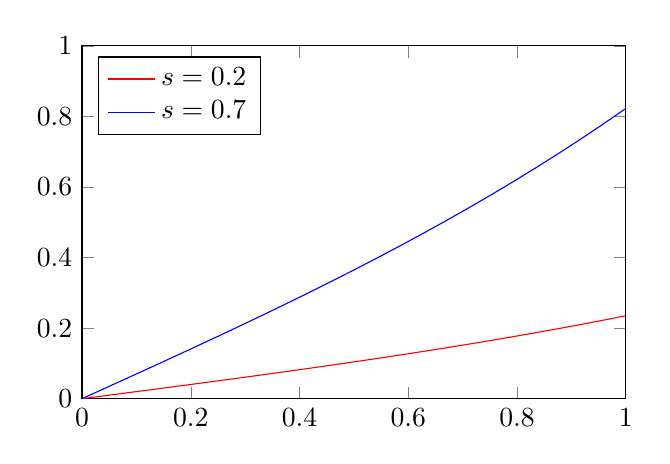
\begin{tikzpicture}
    \begin{axis}[%
    legend pos= north west,
    xmin=0,xmax=1,
    ymin=0,ymax=1,
    width=0.7\textwidth,
    height=0.5\textwidth]
      \addplot[color=red, domain=0:1]{0.2*sinh(x)};
      \addlegendentry{$s=0.2$}
      \addplot[color=blue, domain=0:1]{0.7*sinh(x)};
      \addlegendentry{$s=0.7$}
    \end{axis}
  \end{tikzpicture}
  \caption{Plott av ligning \eqref{eq:ex1a} med forskjellige $s$-verider.}
  \label{fig:s_verdier}
\end{figure}

\noindent Vi ønsker \emph{egentlig} å løse \eqref{eq:ex1eq} med følgende \textbf{rand}betingelser:
\begin{equation}
  y(0) = 0, \; y(1) = 1 \tag{rb}
\end{equation}

I dette tilfellet kan vi, fordi vi kjenner den analytiske løsningen \eqref{eq:ex1a}, se at dette problemet kan løses ved å velge $s=s^*$ slik at $y(1)=s^* \sinh(1)$. Men ettersom vi vanligvis ikke kjenner den analytiske løsningen må vi bruke en annen fremgangsmåte for å finne $s^*$.

For å løse vår ligning må vi velge verdier av $s$ helt til betingelsen $y(1)=1$ er oppfylt. For vilkårlige verdier av $s$ blir $y(1)$ da en funksjon av $s$. Vi starter med å skrive \eqref{eq:ex1eq} som et system:
\begin{align}
  y'(x) &= g(x) \\
  g'(x) &= y(x)
\end{align}

%%%%%%%%%%%%%
% TODO
%%%%%%%%%%%%%


% subsection en_enkel_ligning (end)


\subsection{Løsing av en generell 2. ordens lineær differensialligning} % (fold)
\label{sub:eksempel_l_sing_av_en_2_orden_line_r_differensialligning}
Vi vil løse følgende generaliserte ligning:
\begin{equation}
  y''(x) = p(x)\cdot y'(x) + q(x)\cdot y(x) + r(x) \label{eq:2olgen}
\end{equation}
med randbetingelser
\begin{equation}
  y(a) = \alpha, \; y(b) = \beta \tag{b}
\end{equation}
Starter med å skrive \eqref{eq:2olgen} som et ligningssystem:
\begin{align}
  y'(x) &= g(x) \\
  g'(x) &= p(x)\cdot y'(x) + q(x)\cdot y(x) + r(x)
\end{align}
% subsection eksempel_l_sing_av_en_2_orden_line_r_differensialligning (end)

%%%%%%%%%%%%%
% TODO
%%%%%%%%%%%%%

% section line_re_ligninger (end)


\clearpage
\begin{thebibliography}{1}
  \bibitem{komp} Numeriske beregninger kompendium, \emph{Jan B. Aarseth}
  \bibitem{wolf} Wolfram.com artikkel om løsing av randverdiproblemer: \\ \url{http://reference.wolfram.com/mathematica/tutorial/NDSolveBVP.html}
\end{thebibliography}

\end{document}
